\documentclass[11pt]{article}

\usepackage[margin=0.85in]{geometry}
\usepackage{graphicx}
\usepackage{booktabs}
\usepackage{hyperref}
\usepackage{float}
\usepackage{array}

\title{Yichao Brightfield-to-Fluorescence Mask Model: Partial Training Report}
\author{OrganoidAgent}
\date{May 11, 2026}

\begin{document}
\maketitle

\section{Status}

The previous tmux training run did not finish. It stopped after epoch 20 because a PyTorch
DataLoader worker segfaulted:

\begin{verbatim}
RuntimeError: DataLoader worker (pid 1116658) is killed by signal: Segmentation fault.
YICHAO_SEGMENTATION_FAILED 2026-05-11T09:05:03+08:00 status=1
\end{verbatim}

Therefore this is not a final early-stopped model report. There is no final
\texttt{test\_metrics.json} produced by the normal training script. To still quantify the
run, the saved best checkpoint was evaluated separately with \texttt{num\_workers=0}, which
avoids the worker crash.

\section{Training Setup}

The run trained a mask-only model:

\[
B \rightarrow \hat{M}
\]

where \(B\) is the brightfield organoid crop and \(M\) is a cleaned binary fluorescence
positive mask derived from the fluorescence channel. The model used the original, stricter
mask targets, not the later relaxed masks.

\begin{table}[H]
\centering
\begin{tabular}{ll}
\toprule
Item & Value \\
\midrule
Run root & \texttt{analysis-outputs/yichao\_fluorescence\_segmentation/runs/global\_gated\_unet\_v1} \\
Target root & \texttt{analysis-outputs/yichao\_fluorescence\_segmentation} \\
Input size & \(384 \times 384\) \\
Batch size & 8 \\
Model & Global-gated U-Net with ASPP context \\
Training split size & 6691 crops \\
Validation split size & 1601 crops \\
Test split size & 1088 crops \\
Best checkpoint & epoch 6 \\
Stopped epoch & 20, failed by DataLoader worker segfault \\
\bottomrule
\end{tabular}
\end{table}

\section{Quantification}

The best validation checkpoint was epoch 6. Validation improved early, but the run did not
complete and validation metrics became unstable afterward.

\begin{table}[H]
\centering
\begin{tabular}{lrr}
\toprule
Metric & Validation, best checkpoint & Test, best checkpoint \\
\midrule
Best threshold & 0.300 & 0.600 \\
Best precision & 0.274 & 0.064 \\
Best recall & 0.194 & 0.066 \\
Best F1 & 0.227 & 0.065 \\
Best F0.5 & 0.253 & 0.065 \\
Best IoU & 0.128 & 0.034 \\
Pixel AP & 0.159 & 0.034 \\
Global AUROC & 0.756 & 0.813 \\
Global AP & 0.798 & 0.688 \\
\bottomrule
\end{tabular}
\end{table}

The interpretation is mixed. The global expression score has signal on the test set
(\(\mathrm{AUROC}=0.813\)), so the model is learning image-level information. Pixel-level
mask prediction is poor on the test set (\(\mathrm{F0.5}=0.065\), \(\mathrm{IoU}=0.034\)),
so the model is not reliably localizing expression regions under the original target
definition.

\section{Training Curves}

\begin{figure}[H]
\centering
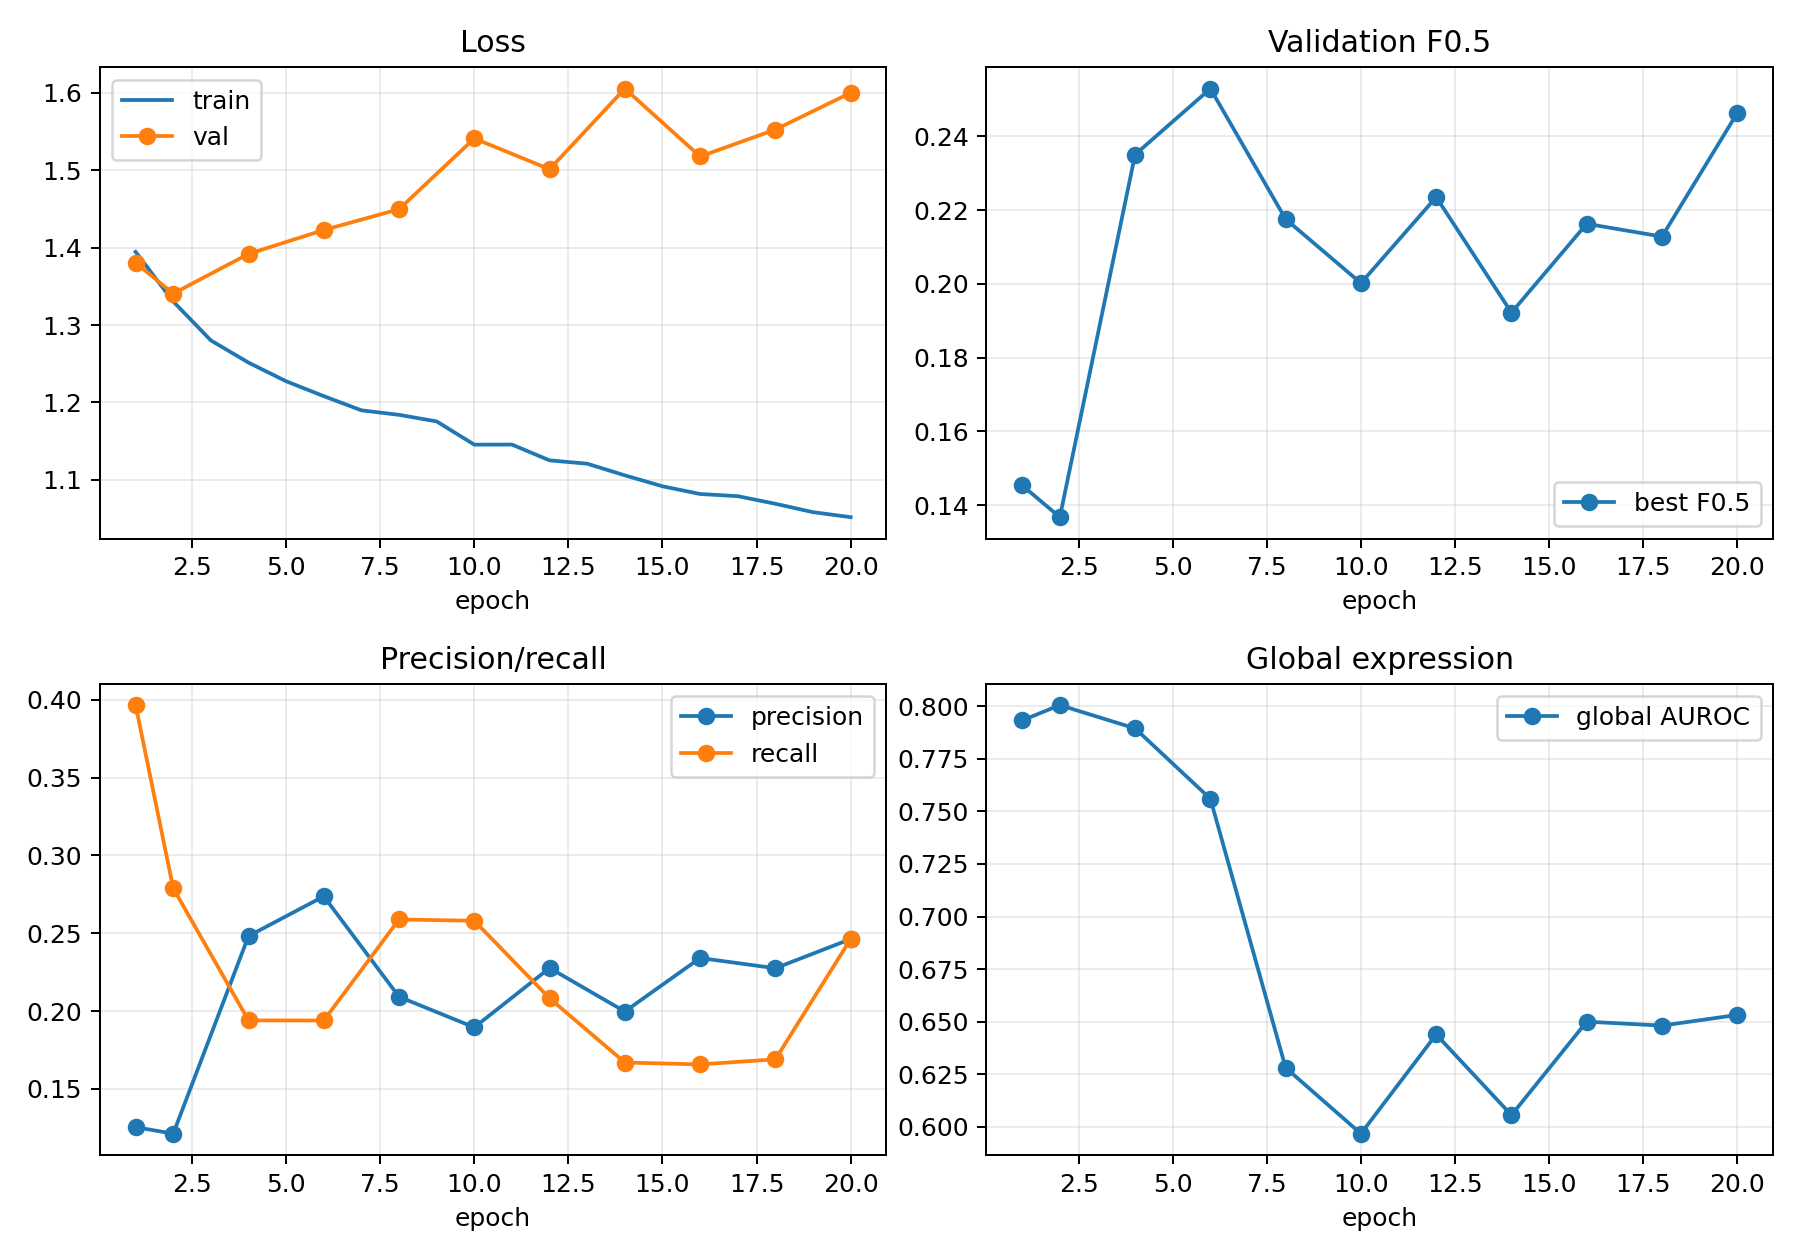
\includegraphics[width=\textwidth]{figures/training_metrics.png}
\caption{Partial training curves until the run failed. Training loss decreased from 1.394
to 1.052, but validation loss increased and validation metrics were unstable.}
\end{figure}

\section{Prediction Visualization}

\begin{figure}[H]
\centering
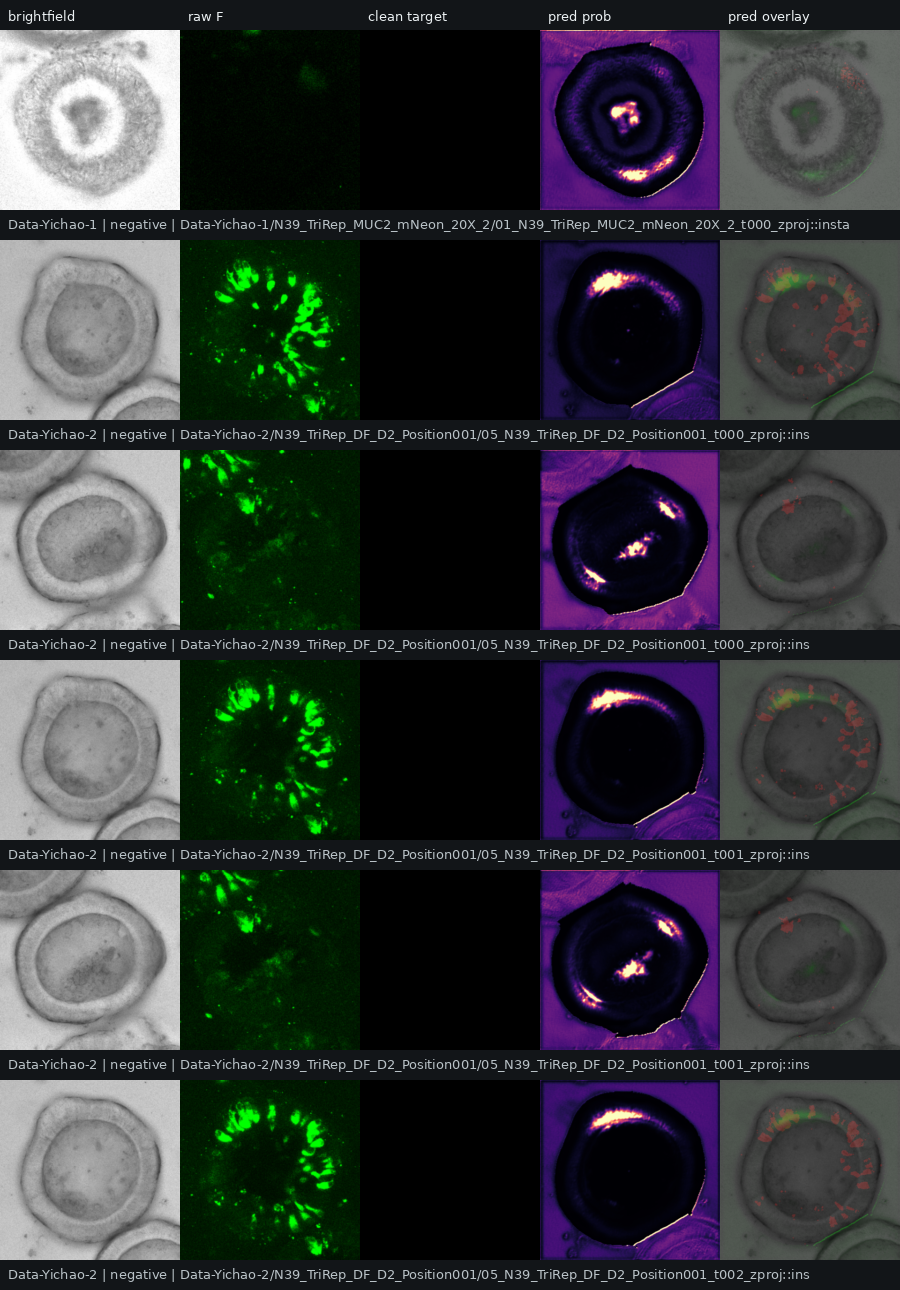
\includegraphics[width=0.86\textwidth]{figures/test_best_checkpoint.png}
\caption{Test-set predictions from the saved best checkpoint. Columns show brightfield,
raw fluorescence, clean target, predicted probability, and overlay. Several fluorescence
positive looking examples are labeled as negative/blank under the original strict target,
which makes this run hard to interpret as a biology-valid model.}
\end{figure}

\section{Target Quality}

The original target masks were intentionally conservative. After visual inspection, they
appear too aggressive for this dataset and miss many real fluorescence-positive regions.
This explains why the model can learn a global signal but struggles to learn reliable
pixel-level localization.

\begin{figure}[H]
\centering
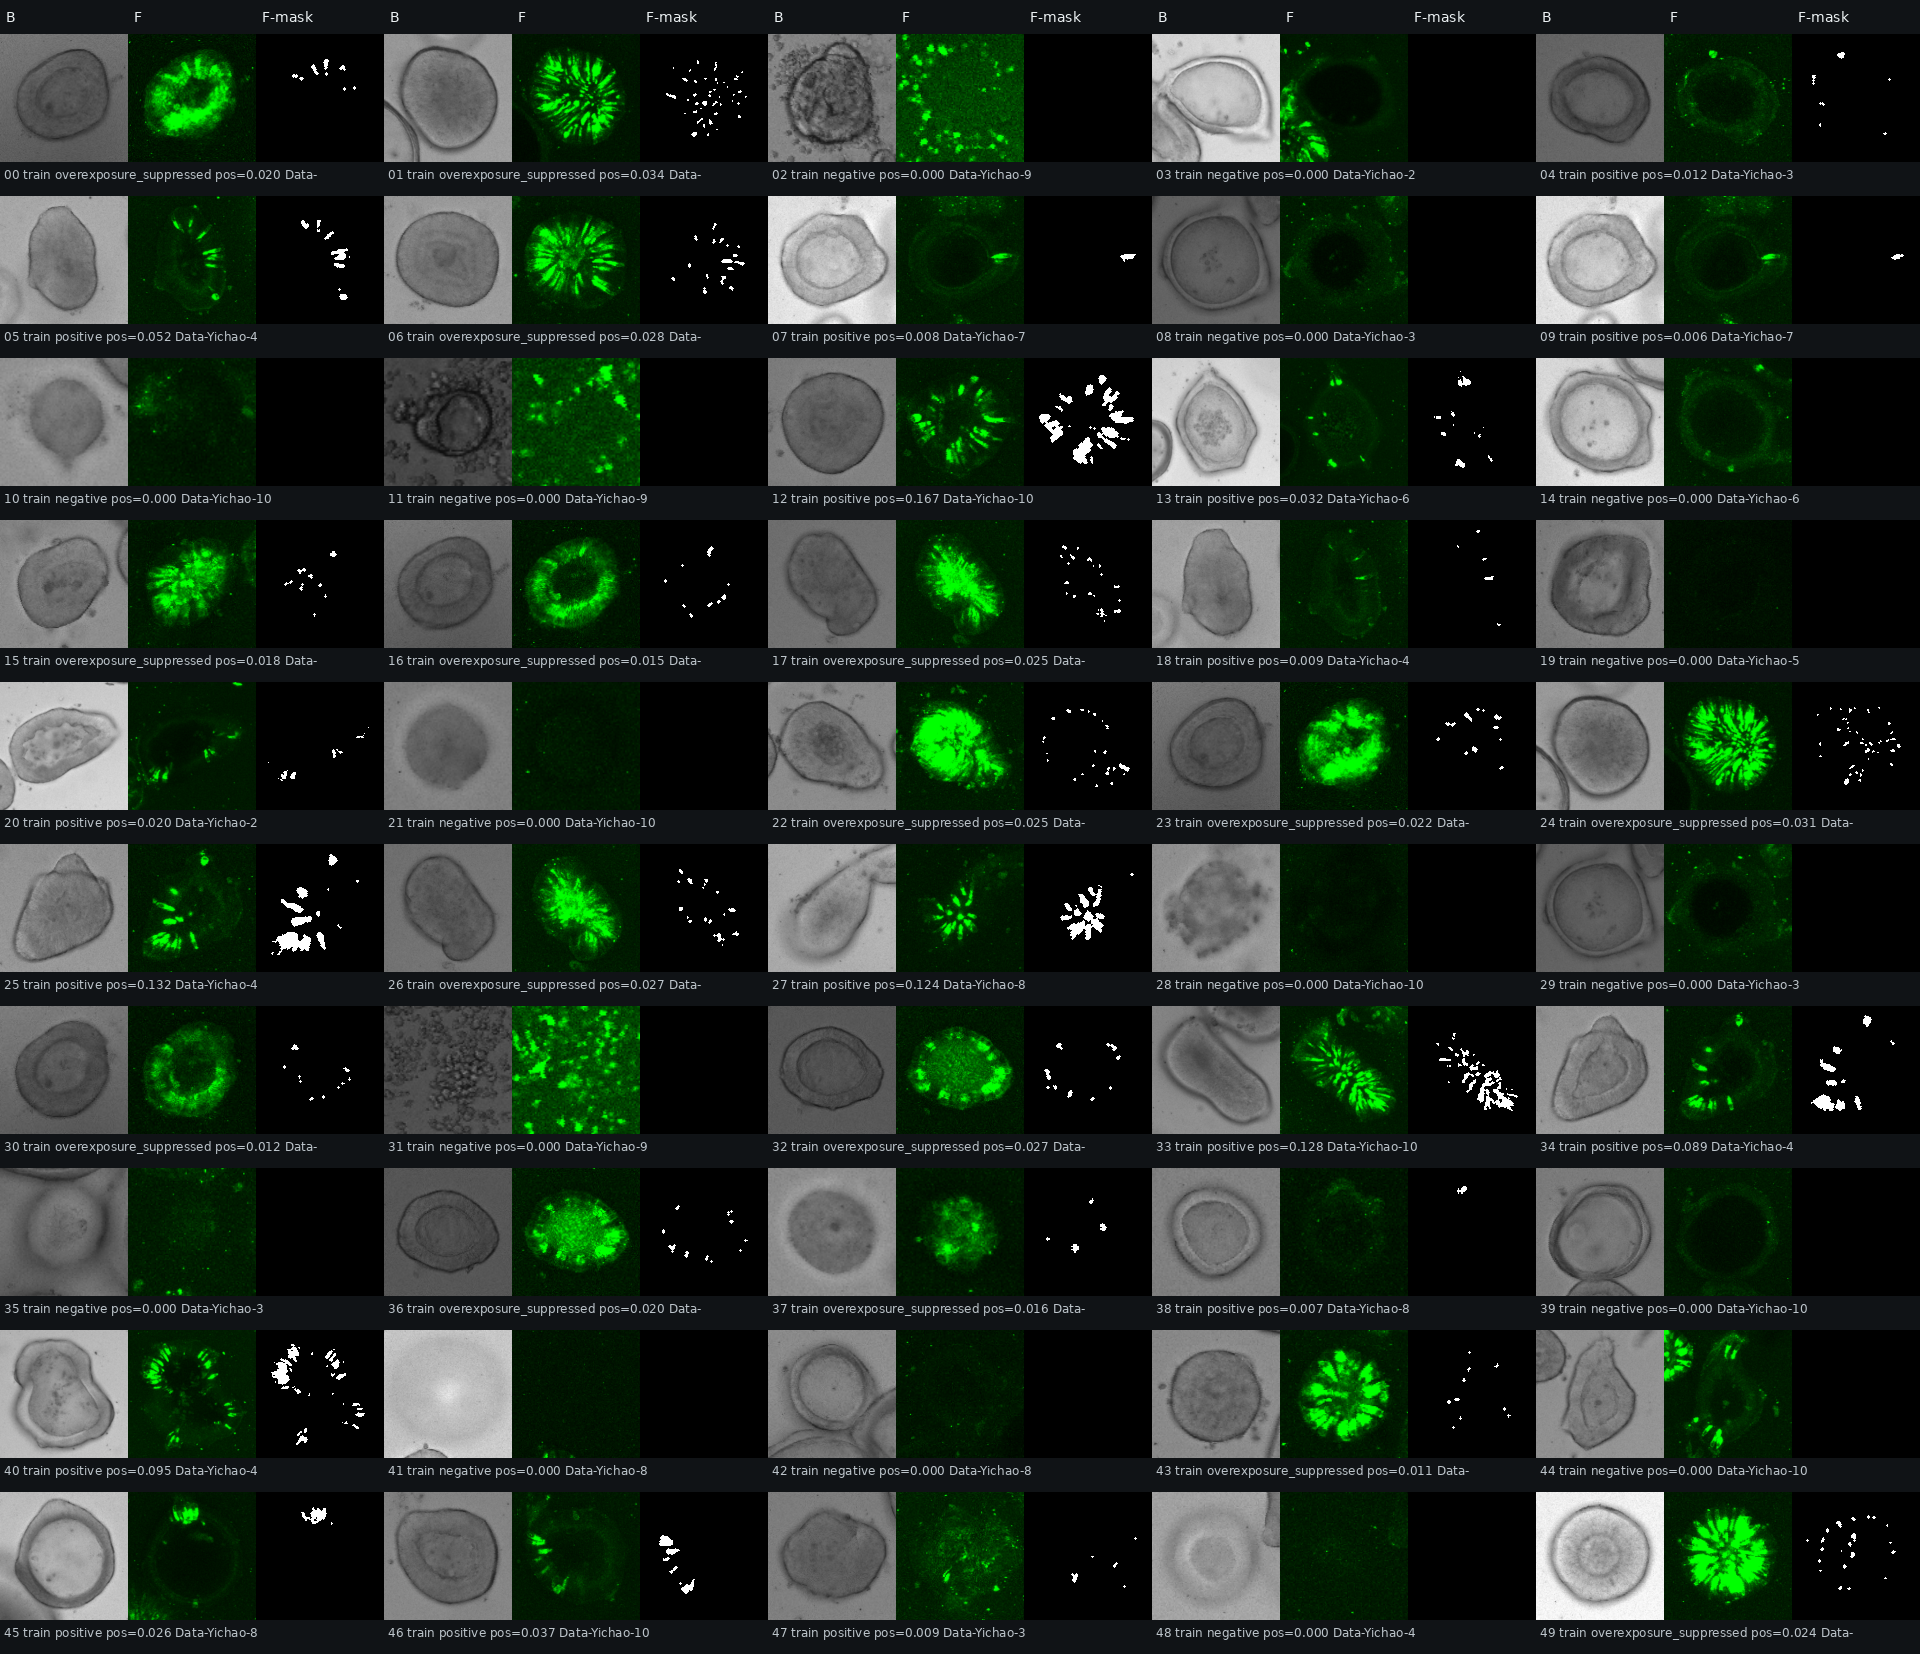
\includegraphics[width=\textwidth]{figures/default_clean_mask_grid.png}
\caption{Original strict clean masks used by the failed run. The masks are sparse and often
miss weak or thin fluorescence signal.}
\end{figure}

A relaxed target generation preset was then added. It lowers the robust fluorescence
thresholds, disables the morphological opening step that removed thin signal, preserves
smaller objects, and keeps full-field overexposure suppression. This relaxed version should
be used for the next training run.

\begin{figure}[H]
\centering
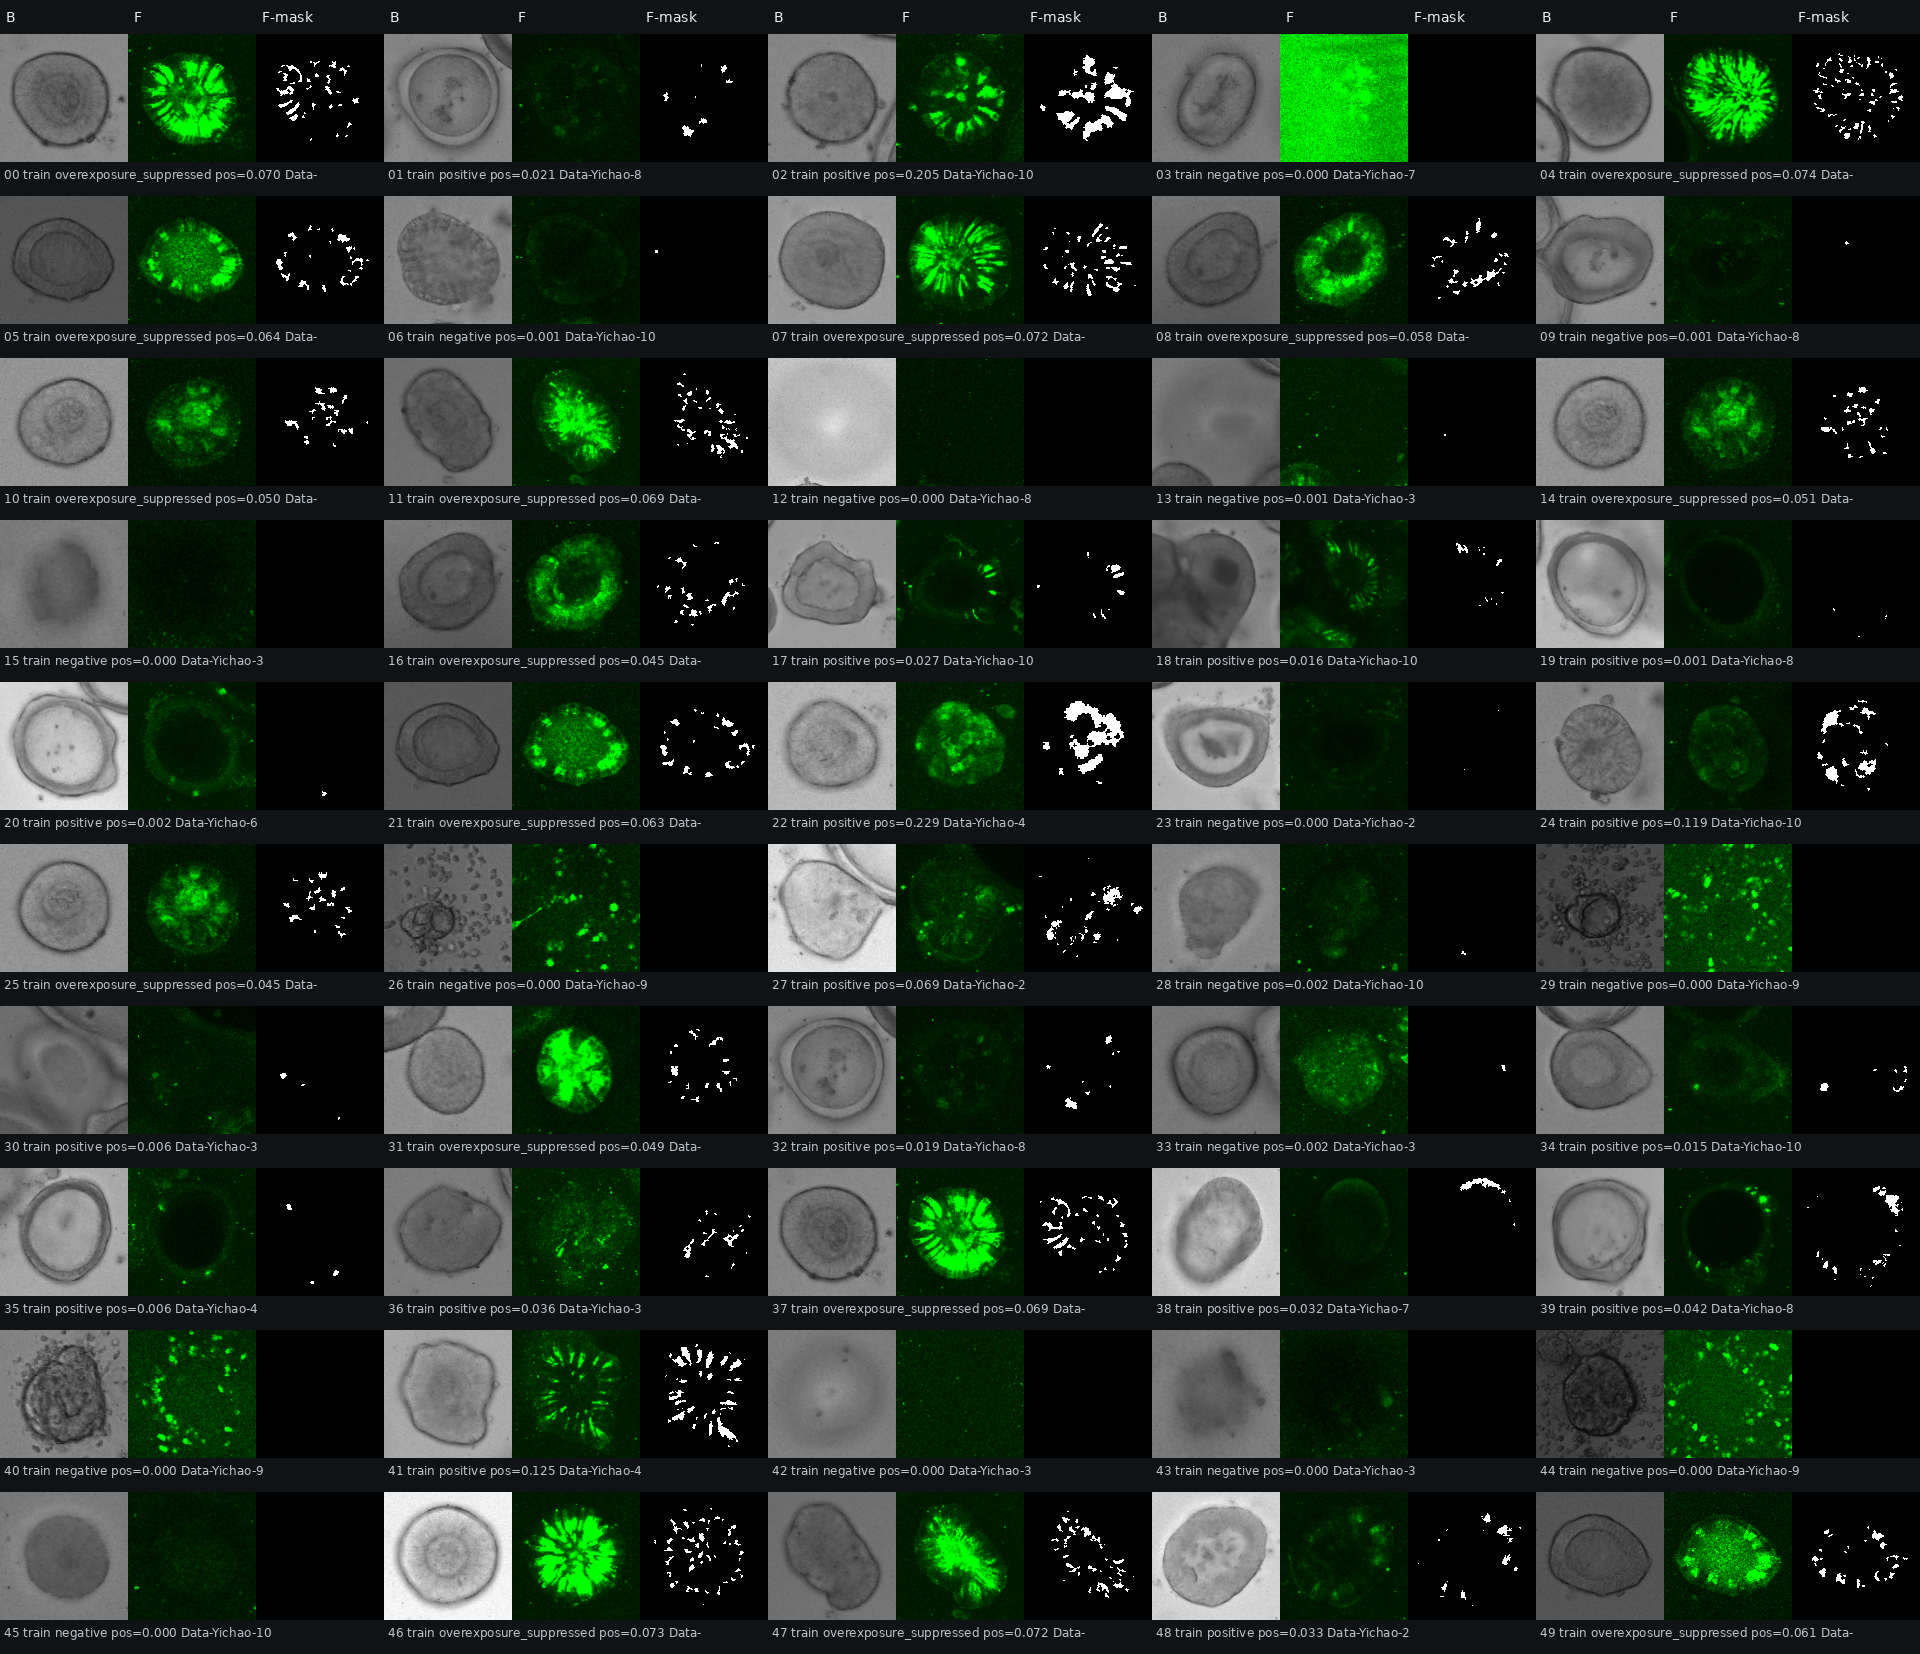
\includegraphics[width=\textwidth]{figures/relaxed_b_f_clean_mask_grid.png}
\caption{Relaxed B/F/mask examples. These targets recover more weak and peripheral signal
while still suppressing many obvious blank or debris-heavy examples.}
\end{figure}

\begin{figure}[H]
\centering
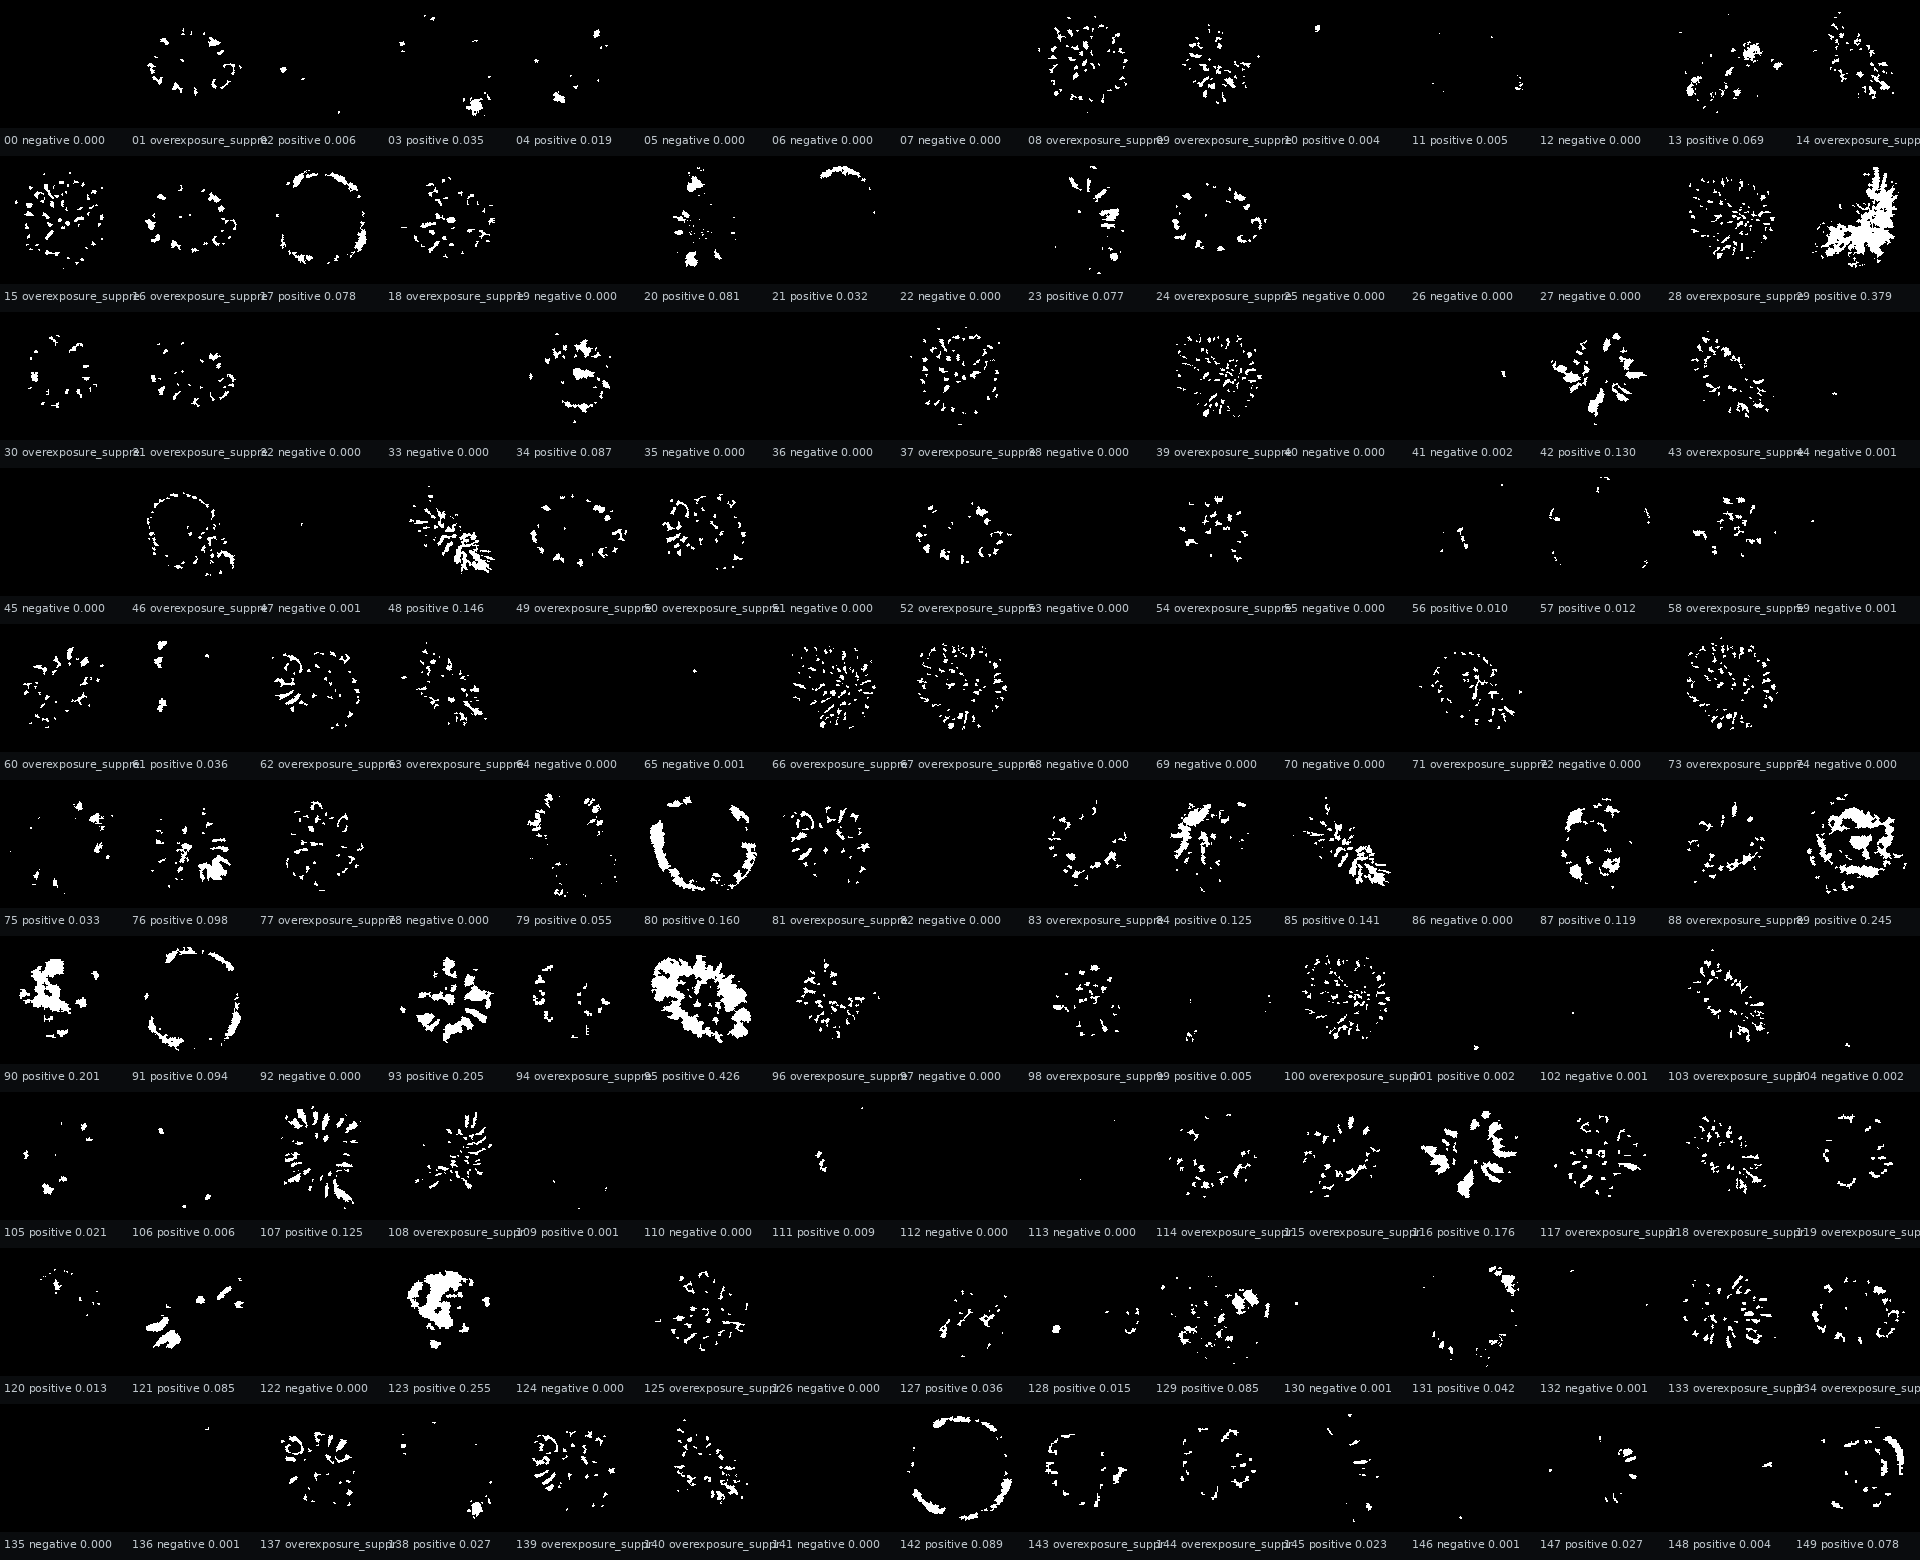
\includegraphics[width=\textwidth]{figures/relaxed_mask_only_grid.png}
\caption{Pure relaxed positive masks. White pixels are the final positive mask. Black
pixels are not positive.}
\end{figure}

\section{Explanation}

The run is best understood as a failed baseline rather than a final result:

\begin{enumerate}
\item The model did learn during training; training loss decreased steadily.
\item Validation mask metrics improved early, with best validation F0.5 at epoch 6.
\item The test pixel-level mask result was weak, so localization did not generalize.
\item The test global AUROC was substantially better than random, so the brightfield still
contains expression-related information at the organoid level.
\item The old target masks were too conservative and sometimes marked real fluorescence as
negative, which creates contradictory supervision.
\item The run failed because a multi-worker DataLoader process segfaulted, not because the
model reached early stopping.
\end{enumerate}

\section{Recommended Next Step}

Do not treat this checkpoint as the final model. The next run should:

\begin{enumerate}
\item Use the relaxed target root:
\texttt{analysis-outputs/yichao\_fluorescence\_segmentation\_relaxed}.
\item Run with \texttt{num\_workers=0} or a safer worker configuration to avoid the
segfault.
\item Use the three-level model design:
\[
B \rightarrow \hat{G}, \quad B \rightarrow \hat{M}, \quad B \rightarrow \hat{A},
\quad \hat{F}=\hat{M}\hat{A}.
\]
\item Select checkpoints by both region metrics and image-level expression metrics.
\end{enumerate}

\end{document}
